\documentclass[../../../analisi-dei-requisiti.tex]{subfiles}

\begin{document}


\subsubsection{AUC3: Creazione organizzazione}%
\label{subs:AUC3}

\begin{figure}[H]
  \centering
  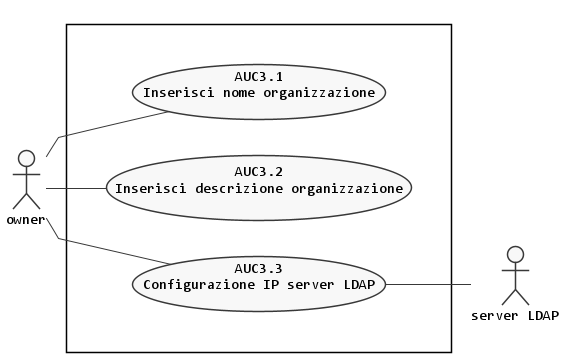
\includegraphics[width=100mm]{creazione-organizzazione.png}
  \caption{AUC3: Creazione organizzazione}%
  \label{fig:AUC3}
\end{figure}

\begin{description}
  \item[Codice:] AUC3;
  \item[Titolo:] Creazione organizzazione;
  \item[Attori primari:] owner;
  \item[Attori secondari:] server LDAP\@;
  \item[Precondizione:] l'organizzazione non deve esistere nella lista di \emph{Stalker};
  \item[Postcondizione:] l'organizzazione viene creata;
  \item[Scenario principale:]
        \begin{enumerate}
          \item sorge la necessità di creare un'organizzazione.
        \end{enumerate}
\end{description}

\subsubsection{AUC3.1: Inserisci nome organizzazione}%
\label{subs:AUC3.1}
\begin{description}
  \item[Codice:] AUC3.1;
  \item[Titolo:] Inserisci nome organizzazione;
  \item[Attori primari:]  owner;
  \item[Precondizione:] il sistema deve rendere disponibile la possibilità di inserire il nome di una nuova organizzazione;
  \item[Postcondizione:] il nome viene opportunamente inserito;
  \item[Scenario principale:]
        \begin{enumerate}
          \item si vuole inserire il nome di un'organizzazione.
        \end{enumerate}

\end{description}

\subsubsection{AUC3.2: Inserisci descrizione organizzazione}%
\label{subs:AUC3.2}
\begin{description}
  \item[Codice:] AUC3.2;
  \item[Titolo:] Inserisci descrizione organizzazione;
  \item[Attori primari:] owner;
  \item[Precondizione:] il sistema deve rendere disponibile la possibilità di inserire una descrizione di una nuova organizzazione;
  \item[Postcondizione:] la descrizione viene opportunamente inserita;
  \item[Scenario principale:]
        \begin{enumerate}
          \item si vuole inserire la descrizione di un'organizzazione.
        \end{enumerate}
\end{description}

\subsubsection{AUC3.3: Configurazione IP server LDAP}%
\label{subs:AUC3.3}
\begin{description}
  \item[Codice:] AUC3.3;
  \item[Titolo:] Configurazione IP server LDAP\@;
  \item[Attori primari:] owner;
  \item[Attori secondari:] server LDAP\@;
  \item[Precondizione:] il sistema deve rendere disponibile la possibilità di configurazione del server LDAP\@;
  \item[Postcondizione:] l'indirizzo IP del server LDAP viene inserito;
  \item[Scenario principale:]
        \begin{enumerate}
          \item si vogliono configurare i dettagli del \glossario{server LDAP} che le applicazioni mobile dovranno utilizzare per collegarsi ad un'organizzazione;
        \end{enumerate}
\end{description}

\subsubsection{AUC4: Eliminazione organizzazione}%
\label{subs:AUC4}
\begin{description}
  \item[Codice:] AUC4;
  \item[Titolo:] Eliminazione organizzazione;
  \item[Attori primari:] gestore;
  \item[Precondizione:] deve essere stata selezionata l'organizzazione da eliminare, presente nella lista di \emph{Stalker};
  \item[Postcondizione:] l'organizzazione viene eliminata;
  \item[Scenario principale:]
        \begin{enumerate}
          \item sorge la necessità di eliminare un'organizzazione;
        \end{enumerate}
\end{description}

\begin{figure}[H]
  \centering
  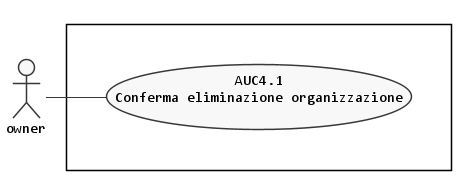
\includegraphics[width=100mm]{eliminazione-organizzazione.png}
  \caption{AUC4: Eliminazione organizzazione}%
  \label{fig:AUC4}
\end{figure}

\subsubsection{AUC4.1: Conferma eliminazione organizzazione}%
\label{subs:AUC4.1}
\begin{description}
  \item[Codice:] AUC4.1;
  \item[Titolo:] Conferma eliminazione organizzazione;
  \item[Attori primari:] gestore;
  \item[Precondizione:] deve essere stata selezionata l'organizzazione da eliminare;
  \item[Postcondizione:] viene confermata l'eliminazione dell'organizzazione;
  \item[Scenario principale:]
        \begin{enumerate}
          \item l'owner visualizza la conferma di eliminazione di un'organizzazione;
        \end{enumerate}
\end{description}

\subsubsection{AUC5: Modifica organizzazione}%
\label{subs:AUC5}

\begin{figure}[H]
  \centering
  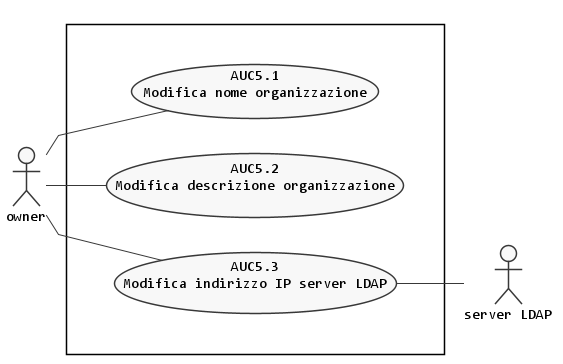
\includegraphics[width=100mm]{modifica-organizzazione.png}
  \caption{AUC5: Modifica organizzazione}%
  \label{fig:AUC5}
\end{figure}

\begin{description}
  \item[Codice:] AUC5;
  \item[Titolo:] Modifica organizzazione;
  \item[Attori primari:] owner;
  \item[Attori secondari:] server LDAP\@;
  \item[Precondizione:] l'owner seleziona l'organizzazione da modificare, presente nella lista di \emph{Stalker};
  \item[Postcondizione:] l'organizzazione viene modificata;
  \item[Scenario principale:]
        \begin{enumerate}
          \item sorge la necessità di modificare un'organizzazione.
        \end{enumerate}
\end{description}

\subsubsection{AUC5.1: Modifica nome organizzazione}%
\label{subs:AUC5.1}
\begin{description}
  \item[Codice:] AUC5.1;
  \item[Titolo:] Modifica nome organizzazione;
  \item[Attori primari:] owner;
  \item[Precondizione:] il sistema deve rendere disponibile la possibilità di modificare il nome di un'organizzazione;
  \item[Postcondizione:] il nome viene opportunamente modificato;
  \item[Scenario principale:]
        \begin{enumerate}
          \item si vuole modificare il nome di un'organizzazione.
        \end{enumerate}
\end{description}

\subsubsection{AUC5.2: Modifica descrizione organizzazione}%
\label{subs:AUC5.2}
\begin{description}
  \item[Codice:] AUC5.2;
  \item[Titolo:] Modifica descrizione organizzazione;
  \item[Attori primari:] owner;
  \item[Precondizione:] il sistema deve rendere disponibile la possibilità di modificare la descrizione di un'organizzazione;
  \item[Postcondizione:] la descrizione viene opportunamente modificata;
  \item[Scenario principale:]
        \begin{enumerate}
          \item si vuole modificare la descrizione di un'organizzazione.
        \end{enumerate}
\end{description}


\subsubsection{AUC5.3: Modifica indirizzo IP server LDAP}%
\label{subs:AUC5.3}
\begin{description}
  \item[Codice:] AUC5.3;
  \item[Titolo:] Modifica indirizzo IP server LDAP\@;
  \item[Attori primari:] owner;
  \item[Attori secondari:] server LDAP\@;
  \item[Precondizione:] il sistema deve rendere disponibile la possibilità di modifica dell'idirizzo IP del server LDAP\@;
  \item[Postcondizione:] l'indirizzo IP del server LDAP viene modificato;
  \item[Scenario principale:]
        \begin{enumerate}
          \item si vuole modificare l'indirizzo IP del server LDAP\@.
        \end{enumerate}
\end{description}

\end{document}
